\chapter{Outline to Evaluation Approach}
\label{chap:evaluation-outline}
\centerline{\rule{149mm}{.02in}}
\vspace{2cm}

One of the project's deliverables is an evaluation of the implemented index structure(s). Multiple evaluations will be performed to guide what needs to be achieved in each iteration of development and determine how efficient the final implementations at the end of the project are. As such, evaluation forms a large part of the project. This section details what measurements will be used to evaluate implementation performance, what the baselines are (i.e. what the implementations will be compared to) and what data will be used for the evaluation.

\section{Performance Measures}

A variety of measurements have been used to evaluate the performance of index structures. Which measurements to use depend on the focus of the research and what problem the specific structure is trying to solve. Section \ref{sec:measuring-efficiency} discusses the ways index structures are commonly evaluated in the literature. This project is aimed towards accelerating index structures both algorithmically and by optimising the implementation itself. The performance analysis tools discussed in Section \ref{sec:development-tools} will be used to produce some of the chosen evaluation measures, which are:

\begin{itemize}
	\item \textbf{Total Execution Time} -- total time it took an operation to execute
	\item \textbf{Cache Hit Rate} -- rate of cache hits to misses ($\frac{\text{\# cache hits}}{\text{\# cache misses}}$)
	\item \textbf{Peak Heap Memory} -- maximum amount of heap memory used at once by the simulation 
	\item \textbf{Total Memory} -- total amount of stack and heap memory used over the entire simulation
	\item \textbf{\# Heap Allocations} -- the amount of system calls made to allocate memory on the heap
	\item \textbf{Speedup Factor} -- increase in speed when compared to another index structure (e.g. evaluation baselines). This is given by $\frac{t_1}{t_2}$, where $t_1$ and $t_2$ are the running times of the two index structures being compared.
\end{itemize}

One assumption being made about the target data is that it is dynamic, meaning points may be inserted or deleted at any time. For query performance, the evaluation will focus on the performance of point queries. Therefore, index structures will be evaluated using the performance of their \textbf{insert}, \textbf{delete} and \textbf{point query} operations.

\section{Timing Operations}
\label{sec:timing-operations}

\textbf{Amortised analysis}, introduced by Tarjan in 1985, is used to analyse the performance of algorithms over a sequence of operations, rather than an individual one \cite{amortised-analysis}. This type of analysis is typically used for algorithms where some operations take longer than others, with the goal of making operations later quicker. The amortised time complexity of an algorithm. Some index structures, particularly self-adjusting ones, have used this to bound the running time of their operations, such as the Splay tree, Quadtreap and Splay Quadtree \cite{splay-tree, quadtreap, splay-quadtree}.

This project will use a similar concept for measuring the execution time of the structures. Instead of measuring the time of a single operartion, the times of many thousands of operations will be measured. This is to get an idea on what the runtime of an operation is on average, over a sequence of operations. This prevents single, slow operations from causing the execution time to appear worse, or short operations making the performance appear better. A typical performance test therefore has the following steps:
\begin{enumerate}
	\item \textbf{Initial Build} -- incrementally build structure by adding each point in test dataset one-by-one
	\item \textbf{Query Points} -- query each point in the dataset, which should not be in the structure
	\item \textbf{Delete Points} -- delete each point in the dataset from the structure until it is empty
\end{enumerate}
Using this process allows the runtime of large numbers of \texttt{insert}, \texttt{delete} and point query operations to be measured. Any performance tests of sequences of operations will be performed twice, and the recorded time will be the \textit{average} of the two times.

By interleaving \texttt{insert} and \texttt{delete} operations with a number of point queries, more insight can be gained into how well the implementations perform in real applications that use dynamic data structures, where the pattern of operations is less straightforward. The performance of the implementations on interleaved operations may be different from the test process described previously due to cache coherency. The contents of the cache may change frequently due to different operations being performed consecutively, potentially causing a greater number of cache misses.

The term \textbf{operation list} will be used to refer to a sequence of operations. Each operation will either be an \texttt{insert}, \texttt{delete} or point query, and will be paired with a $d$-dimensional point. These points will be pulled from the datasets described in the next section. Two main operation lists will be used for testing with a given dataset. The first, called \textbf{Insert-Query-Delete}, inserts each point in the dataset, then queries each point and finally deletes each point. The total execution time of each operation type will be measured. The second operation list, \textbf{Random Operations}, contains randomly generated interleaved operations using points taken from the target dataset and points \textit{not present} in the dataset. This is being used to measure how well the structures perform in scenarios that may occur if the structure was used in a real application, as it contains interleaved operations and queries with non-existent points.

% TODO: mention trace of Joint Contour Net behaviour that will be used to see how the index structures perform with a real application -- AND TO SEE HOW INTERLEAVED OPERATIONS

\section{Datasets}
\label{sec:datasets}

Both synthetic, artificially generated data and a real dataset will be used for the evaluation. Three types of random \textbf{synthetic} datasets will be generated, which are uniformly distributed, skewed and clustered. All generated points are in $[0,1]^d$. Multiple instances of these datasets will be used, with varying numbers of dimensions.. Using such datasets was inspired by Wang et al. and Berchtold et al., who used similar datasets to evaluate the performance of the PK-tree and pyramid tree respectively \cite{pk-tree, pyramid-tree}. The reason for testing the index structures with these datasets is that the variety of point distributions and number of dimensions should tease out which data the implementations struggle with and which they work well at.

The synthetic data was generating randomly using the \texttt{boost::random} library and the Mersenne twister pseudorandom number generator (PRNG) \cite{mersenne-twister}.  The Mersenne twister passes ``stringent statistical tests" of randomness, including diehard \cite{mersenne-twister}. \texttt{boost::random} was chosen over using the C standard library function \texttt{rand()} because the latter is platform-dependant, so it is know as to what underlying PRNG will be used and if it passes these stastical tests.

Figure \ref{fig:synthetic-data} shows 2D randomly generated points using uniform, skewed and clustered distributions. Skewed data was generated by applying a power to the number. Let $p$ be a generated point. Since $0 \leq p_i \leq 1$ for all $i \in \lbrace 1, ..., d \rbrace$, this means $p_i^e \leq p_i$ for all $e \geq 1$. This makes smaller values more likely, generating a skewed distribution of points. $e = 1.5$ was used for all skewed datasets generated. The clustered datasets contain two clusters of points, each contained within the hypercubes $[0,0.5]^d$ and $[0.7,0.8]^d$.

\begin{figure}
		\begin{center}
			\begin{subfloat}[Uniform Distribution\label{fig:uniform-distribution}]{%
				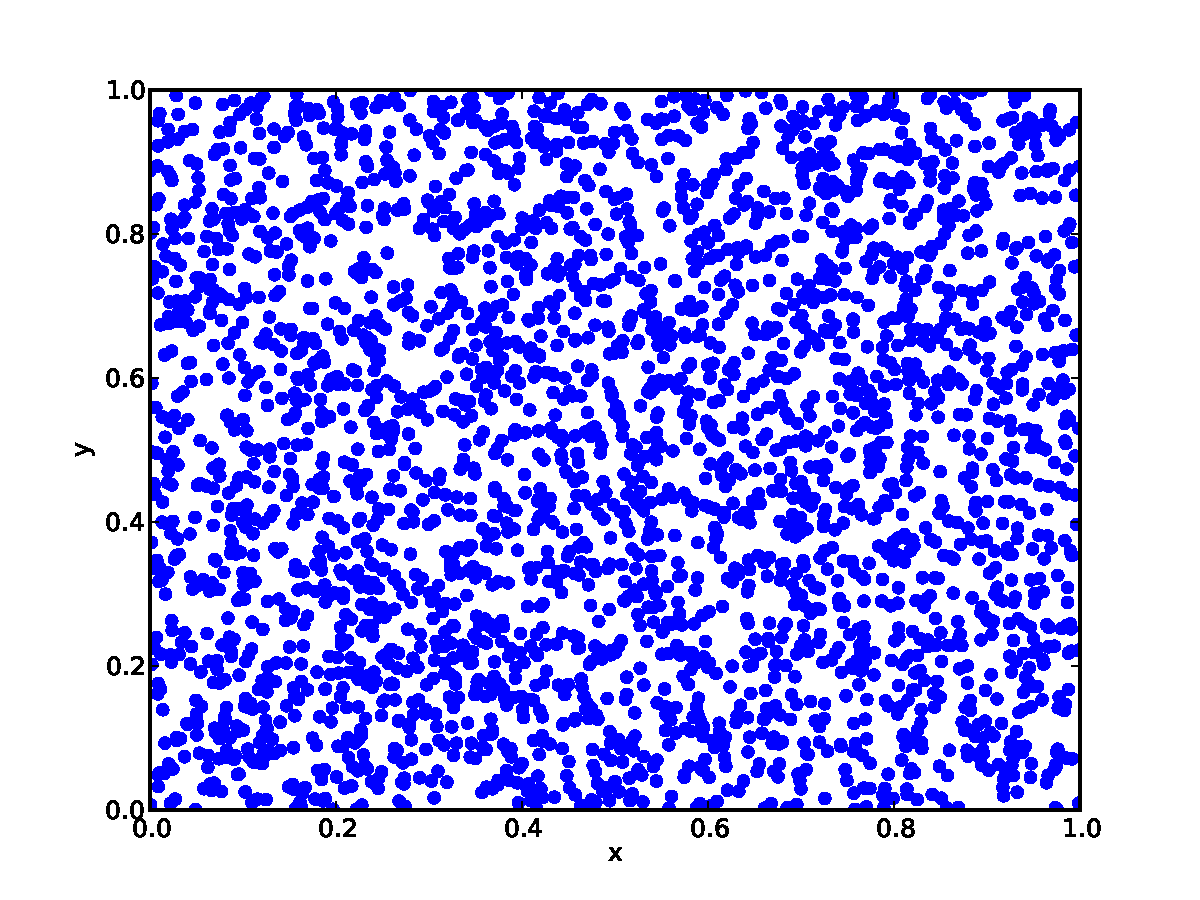
\includegraphics[scale=0.25]{figures/uniform_distribution.pdf}
			}
			\end{subfloat}~
			\begin{subfloat}[Skewed Distribution\label{fig:skewed-distribution}]{%
				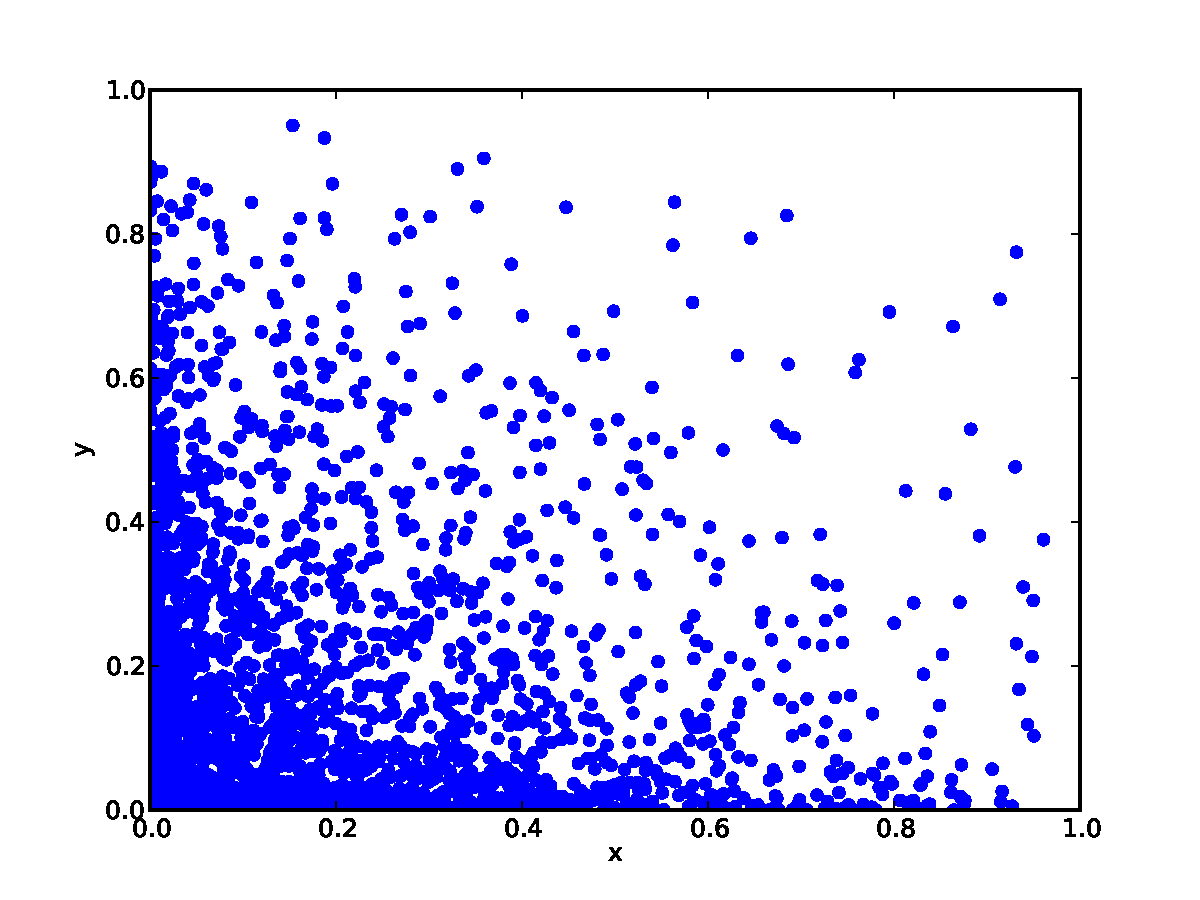
\includegraphics[scale=0.25]{figures/skewed_distribution.pdf}
			}
			\end{subfloat}~
			\begin{subfloat}[Clustered Distribution\label{fig:clustered-distribution}] {%
				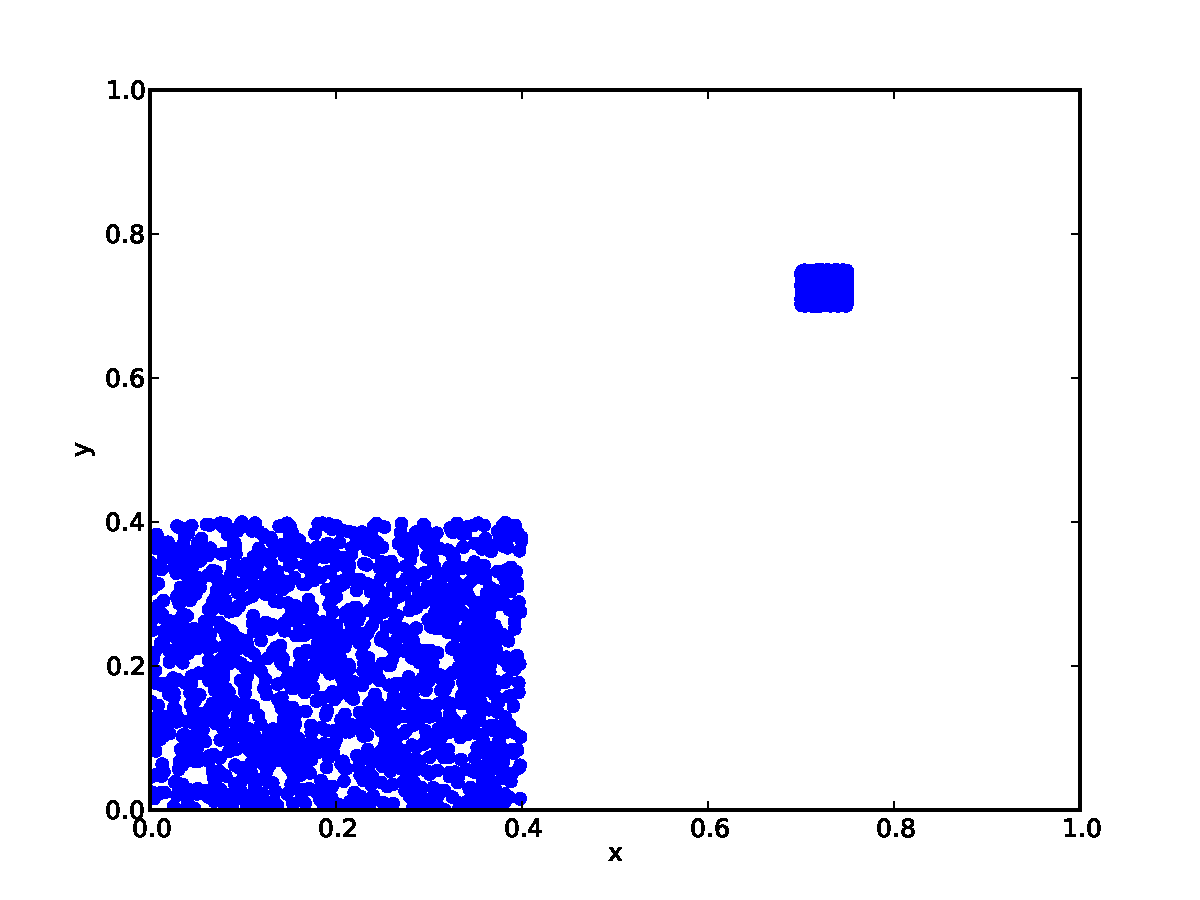
\includegraphics[scale=0.25]{figures/clustered_distribution.pdf}
			}
			\end{subfloat}			  
		\end{center}

		\caption{Three Types of Synthetic Dataset Used For Evaluation, with 3000 Points Each}
		\label{fig:synthetic-data}
\end{figure}

The real dataset being used for the evaluation is the result of an \textbf{astrophysics turbulence simulation}, where a $600 \times 248 \times 248$ regular mesh was used to simulate ``three-dimensional radiation hydrodynamical calculations of ionization front instabilities" \cite{astrophysics-dataset}. Figure \ref{fig:ionisation-front-instabilities} shows an example of a visualisation generated using a 2D slice of the data. Each point of the mesh has ten scalar fields, which include particle density, temperature and eight chemical species. 200 timesteps were recorded, each being approximately 126 to 128 years apart \cite{astrophysics-dataset}. For each evaluation, only \textbf{one timestep} of the simulation will be used at a time. Since some of the timesteps have different distributions, multiple tests with different timesteps may be performed.

\begin{wrapfigure}[12]{r}{0.4\textwidth}
	\vspace{-20pt}
	\begin{center}
		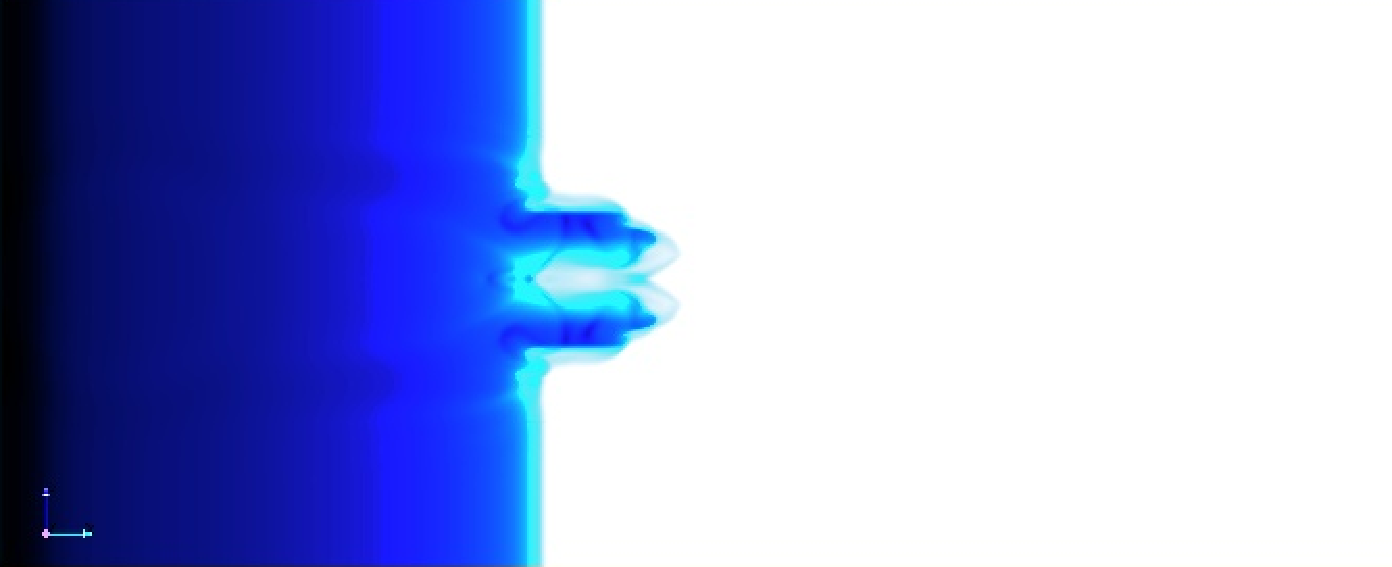
\includegraphics[scale=0.2]{figures/ionisation_front_instabilities.pdf}
	\end{center}
	\vspace{-20pt}
	\caption{Shadow Instability Forming in One 2D Slice Through the Astrophysics Dataset Over Time \cite{astrophysics-dataset}}
	\label{fig:ionisation-front-instabilities}
\end{wrapfigure}

The astrophysics was chosen because it is large (almost 37 million points) and has a high number of dimensions (10). The core focus of the project is high-dimensional data, so this data will provide a true test of how well the implementations perform with real instances of such data. The original dataset has a large number of points. For intermediate evaluations, it was decided to use smaller instances of this dataset for performance tests. Sampling a sub-region of the grid or uniformly sampling to create a dataset with a smaller resolution may introduce \textit{bias} in the data, which affects the evaluation. Therefore, smaller instances of the dataset are generated by randomly picking $n$ points from the original dataset, discarding and picking other points whenever a point that has already been sampled was chosen. By the law of large numbers\footnote{\url{http://en.wikipedia.org/wiki/Law_of_large_numbers}}, as $n$ is increased, the smaller dataset tends to being more representative of whole dataset, making this method statistically fairer.

% TODO: why choose 16?
% TODO: why 100??
% TODO: mentino skew in average runtime and say why it's a problem?
Multiple synthetic datasets with 10,000 points have been generated for each distribution, with varying numbers of dimensions. Tests using these datasets will measure the \textit{total} runtime of the operations, as the number of operations is fixed, meaning a fair comparison can be made. The structures will also be measured against data of varying size. 500,000 randomly generated points with a uniform probability distribution has been generated, which will be sampled to construct each dataset. The large dataset has 16 dimensions, which was chosen to match the tests performed by Berchtold et. al for their Pyramid Tree in \cite{pyramid-tree}. Since the number of operations is dependant on the number of points in the dataset, which varies, the \textit{average} runtime of an operation will be measured. This allows a more fair comparison between operation times of each structure to be made as the dataset size increases. The Insert-Query-Delete operation list will be used for all of these datasets. 

Timestep 100 of the astrophysics turbulence simulation will be used with a varying number of points, with both the Insert-Query-Delete and Random Operations lists. Again, the average runtime of operations will be measured Table \ref{tab:operation-lists} shows the operation lists that will be used for evaluation, which datasets the points will be pulled from, the different values the varying parameter (dimension or dataset size) will have and what performance measure will be used for an operation.

\begin{table}
	\centering
	\makebox[\textwidth][c]{%
	\begin{tabular}{|p{3.5cm}|p{3cm}|p{3.5cm}|p{4cm}|p{4cm}|}
		\hline
		\textbf{Operation List} & \textbf{Distribution(s)} & \textbf{Varying Parameter} & \textbf{Parameter Values} & \textbf{Performance Measure} \\
		\hline
		Insert-Query-Delete & Uniform, Skewed, Clustered & Dimension & 1, 2, 3, 5, 8, 10, 30, 50, 100, 200 & Total Runtime \\
		Insert-Query-Delete & Uniform & Input Size & 10, 100, 1,000, 5,000, 10,000, 50,000, 100,000, 500,000 & \parbox[t]{3in}{Average Operation\par Runtime \strut} \\
		Insert-Query-Delete & \parbox[t]{3in}{Astrophysics\par($t = 100$)\strut} & Input Size & 10, 100, 1,000, 5,000, 10,000, 50,000, 100,000, 500,000 & \parbox[t]{3in}{Average Operation\par Runtime \strut} \\
		Random Operations & \parbox[t]{3in}{Astrophysics\par($t = 100$)\strut} & Input Size & 10,000, 100,000, 500,000 & \parbox[t]{3in}{Average Operation\par Runtime \strut} \\
		\hline
	\end{tabular}}%
	\caption{Operation Lists Used for Main Evaluation}
	\label{tab:operation-lists}
\end{table}

\section{Baselines}

There is little use in measuring the performance of the implemented index structures for the purposes of evaluation if there is nothing to compare the results to. As such, two baseline index structure implementations will be developed -- \textbf{sequential scan} and the \textbf{PR octree} (see Section \ref{sec:recursive-partition-structures}). The reason for choosing sequential scan as a baseline is that it's the na\"{i}ve brute-force approach to performing search. The PR octree is the basis of many index structures, both old and new. Thus, the structure is well-known in the field and makes a suitable baseline.

These baselines have been developed in C++ to match the technology used to develop the initially implemented index structure.

\section{Timing}

TODO: different timing mechanisms, advantages and disadvantages